% !TeX root = RJwrapper.tex
\title{corVis: An R Package for Visualising Associations and Conditional
Associations}
\author{by Amit Chinwan and Catherine Hurley}

\maketitle

\abstract{%
Correlation matrix displays are important tools to explore multivariate
datasets. These displays with other measures of association can
summarize interesting patterns to an analyst and assist them in framing
questions while performing exploratory data analysis. In this paper, we
present new visualisation techniques to visualise association between
all the variable pairs in a dataset in a single plot, which is something
existing displays lack. Also, we propse new methods to visualise
relationship among variable pairs using conditioning. We use different
layouts like matrix or linear for our displays. We use seriation in our
displays which helps in highlighting interesting patterns easily. The R
package \texttt{corVis} provides an implementation.
}

\hypertarget{section-1-introduction}{%
\section{Section 1: Introduction}\label{section-1-introduction}}

Correlation matrix display is a popular tool to visually explore
correlations among variables while performing Exploratory Data Analysis
(EDA) on a multivariate dataset. Popularized by
\citet{friendly2002corrgrams} as corrgram, these displays are produced
by first calculating the correlation among the variables and then
plotting these calculated values in a matrix display. With effective
ordering techniques, these displays quickly highlight variables which
are highly correlated and an analyst interested in building a predictive
model could use these displays to remove correlated variables and avoid
multicollinearity.

The correlation displays are generally used with one of the Pearson's,
Spearman's or Kendall's correlation coefficient and are therefore
limited to quantitative variables. An analyst can use one-hot encoding
of the qualitative variables in order to use these displays but will
need to deal with the high dimensions as a result of the encoding. In
addition to the dimensionality problem, it is not easy to assess the
overall correlation when using the one-hot encoding. The existing
methods to quickly explore association among qualitative variables in a
dataset include using proportions or counts with different graphical
displays like boxplots or barplots. Using association measures for
qualitative pairs similar to correlation for quantitative pairs will
help in summarizing the relationship, which then can be displayed like
the correlation displays.

Tukey and Tukey introduced scagnostics which are measures for
scatterplots \citep{tukey1985computer}. Along with scagnostics, they
proposed a scagnostics scatterplot matrix which is a visual display to
explore and compare these measures for all the variable pairs in a
dataset. By comparing multiple measures at once, the unusual variable
pairs could be identified and looked at in more detail. In a similar
manner, a display comparing association measures will help in finding
interesting variable pairs. Many association measures have been proposed
to summarize different types of relationships. The most commonly used
measure is Pearson's correlation coefficient which captures any linear
trend present between the variables. Other popular measures include
Kendall's or Spearman's rank correlation coefficient which are
non-parametric measures and looks for monotonic relationship. Distance
correlation \citep{szekely2007measuring} is an important measure useful
in exploring non-linear relationships. The information theory measure
maximal information coefficient (MIC) \citep{reshef2011detecting} is
capable of summarizing complex relationships. With effective displaying
techniques, the multiple measures of association provide a comparison
tool that assist an analyst to reveal structure present in the data.

Small multiples (or Trellis display) is a simple yet powerful approach
to compare partitions of data and understand multidimensional datasets
\citep{tufte1986thevisual}. The display is produced by splitting the
data into groups by a conditioning variable and then plotting the data
for each group. Such displays allow analysts to quickly infer about the
impact of the conditioning variable. A similar idea applied to displays
of association measures (correlation plot) will help uncover underlying
patterns in the data. One such pattern is Simpson's paradox which can be
detected by comparing Pearson's correlation for data at overall level
versus individual levels of the conditioning variable.

In this paper, we propose extensions of the correlation plot and new
visualizations which look at variables of mixed type, multiple
association measures and conditional associations. These displays are
implemented in the R package \CRANpkg{corVis}. The next section provides
a review of existing packages which deal with correlation displays and a
quick background on association measures and the packages used for
calculating them. Then we describe our approach to calculate the
association measures, followed by visualizations of associations and
conditional associations. We conclude with a summary and future work.

\hypertarget{section-2-background}{%
\section{Section 2: Background}\label{section-2-background}}

In this section we provide a brief review of existing packages used for
correlation displays and association measure calculation.

\hypertarget{section-2.1-literature-review-on-correlation-displays}{%
\subsection{Section 2.1: Literature Review on Correlation
Displays}\label{section-2.1-literature-review-on-correlation-displays}}

According to \citet{hills1969looking}, the first and sometimes only
impression gained by looking at a large correlation matrix is its
largeness. In order to explore a large correlation matrix
\citet{hills1969looking} proposed a QQ plot of the entries of the
correlation matrix. According to \citet{murdoch1996graphical}, they
proposed a more effective display for exploring a large correlation
matrix. \citet{murdoch1996graphical} replaced the entries in a
correlation matrix by an ellipse where the parameters of ellipse were
scaled to the correlation value. These displays are called as
correlation matrix displays.

The correlation matrix display is an important tool to explore
association among variables in a multivariate analysis. The display was
made popular by \citet{friendly2002corrgrams} who called them corrgrams,
wherein he rendered the correlation values of \(p\) numeric variables in
a \(p \times p\) matrix layout with shaded squares, bars, ellipses, or
circular `pac-man' symbols. The main goal of these displays is to render
the correlation patterns in a dataset.

Table \ref{tab:corrdisplay-packages} provides a list of packages
available in R which either calculate correlations, visualise
correlations or both. The displays provided by each of the packages are
listed, as are the correlations or associations calculated, in
particular whether association measures are provided for factor
variables or mixed numeric-factor pairs. We also summarise whether
packages provide conditional displays of association, by which we mean
displays for each of the levels of a categorical variable.

The R package \CRANpkg{corrplot} \citep{corrplot2021} provides an
implementation of the \citet{friendly2002corrgrams} paper. It serves as
a visual exploratory tool for correlation matrices and includes various
variable ordering methods which place highly-correlated pairs of
variables nearby, making it easier to quickly identify groups of
variables with high mutual correlation.

The package \CRANpkg{corrr} \citep{corrr2020} organises correlations as
tidy data, so leveraging the data manipulation and visualisation tools
of the \CRANpkg{tidyverse} \citep{tidyverse}. In addition to various
matrix displays, the package offers network displays where
line-thickness encodes correlation magnitude, with a filtering option to
discard low-correlation edges.

The package \CRANpkg{corrgrapher} \citep{corrgrapher} calculates a
comparable correlation coefficient for numeric pairs, mixed pairs and
categorical pairs of variables by using the \(p\)-values from Pearson's
correlation test, Kruskal's test and Chi-squared test respectively.
These coefficients are then plotted using a network plot where the nodes
close to each other have high correlation magnitude, edge thickness
encodes the absolute correlation value and edge color indicates the sign
of correlation.

The package \CRANpkg{linkspotter} \citep{linkspotter} offers a variety
of association measures (list some) in addition to correlation, where
the measure used depends on whether the variables are both numerical,
categorical or mixed. The results are visualized in a network plot,
which may be packaged into an interactive shiny application.

We include our own package corvis in the table, which has new features
not available elsewhere, in particular simulaneous display of multiple
association measures, and association displays stratified by levels of a
grouping variable. This will be described further in the following
section.

There have been other extensions to correlation displays which are
useful when dealing with high dimensional datasets.
\citet{buja2016visualization} proposed Association Navigator which is an
interactive visualization tool for large correlation matrices with upto
2000 variables. The R package \CRANpkg{scorrplot} \citep{scorr} produces
an interactive scatterplot for exploring pairwise correlations in a
large dataset by projecting variables as points and encoding the
correlations as space between these points. The package provides a
functionality to update variable of interest which creates tour of the
correlation space between different projections of the data.

The R package \CRANpkg{correlationfunnel} offers a novel display which
assists in feature selection in a setting with a single response and
many predictor variables. All numeric variables including the response
are binned. All (now categorical) variables in the resulting dataset are
one-hot encoded and Pearson's correlation calculated with the response
categories. The correlations are visualised in a dot-plot display, where
predictors are ordered by maximum correlation magnitude. Correlations
between one-hot encoded variables are challenging to interpret,
especially as the number of levels increase. In corVis we offer a
similar dot-plot display, but showing multiple correlation or
association measures, or alternatively measures stratified by a grouping
variable.

\begin{Schunk}
\begin{table}

\caption{\label{tab:corrdisplay-packages}List of the R packages dealing with correlation or correlation displays with information on whether the plots display multiple measures, conditional display of measures and mixed variables in a single plot}
\centering
\begin{tabular}[t]{lllll}
\toprule
Package & Display & MultipleMeasures & ConditionalPlot & MixedVariables\\
\midrule
corrplot & heatmap &  &  & \\
corrr & heatmap/network &  &  & \\
corrgrapher & network &  &  & \\
linkspotter & network &  &  & Yes\\
correlation & heatmap/network &  &  & \\
\addlinespace
corVis & heatmap/matrix/linear & Yes & Yes & Yes\\
\bottomrule
\end{tabular}
\end{table}

\end{Schunk}

\hypertarget{section-2.2-literature-review-on-association-measures}{%
\subsection{Section 2.2: Literature Review on Association
Measures}\label{section-2.2-literature-review-on-association-measures}}

An association measure can be defined as a numerical summary quantifying
the relationship between two or more variables. For example, Pearson's
correlation coefficient summarizes the strength and direction of the
linear relationship present between two numeric variables and is in the
range \([-1,1]\). Kendall's or Spearman's rank correlation coefficient
are other popular measures which assess montonic relationship among two
numeric variables and are in the range \([-1,1]\). As these measures are
limited to linear or monotonic relationships, there's a need to use
association measures which can capture complex relationships (like
periodic). The distance correlation coefficient
\citep{szekely2007measuring} is one such measure which looks for the
non-linear association between two numeric variables and summarizes it
in \([0,1]\). Similarly, MIC \citep{reshef2011detecting} is capable of
summarizing non-linear as well as periodic relationships between numeric
variables. In addition to association measures for numeric variables,
association measures for ordinal or nominal or mixed variables will help
an analyst in exploring a multivariate dataset. \citet{taha201673}
provides an overview of the association measures used for categorical or
mixed data.

We use multiple association measures in a single display for different
variable pairs which serves as a comparison tool while exploring
association in a dataset and assist in identifying unusual variable
pairs. These multiple measures can be displayed in a scatterplot matrix
similar to what \citet{tukey1985computer} proposed. They suggested that
scatterplot matrix of the scagnostics measures, which are measures
summarizing a scatterplot, can be used to identify unusual scatterplots
or variable pairs. \citet{wilkinson2005graph} used this idea with their
graph-theoretic scagnostic measures to highlight unusual scatterplots.
Similarly, \citet{kuhn2013applied} have used this idea in a predictive
modeling context. They have produced a scatterplot matrix of the
measures between the response and continuous predictors such as
Pearson's correlation coefficient, pseudo-\(R^2\) from the locally
weighted regression model, MIC and Spearman's rank correlation
coefficient to explore the predictor importance during feature selection
step. These displays show the importance of comparing multiple
association measures at once for different variable pairs. In this
paper, we propose different visualization techniques to compare multiple
association measures for all the variable pairs in a dataset which can
assist a user in finding interesting patterns.

\hypertarget{section-3-introducing-corvis}{%
\section{Section 3: Introducing
corVis}\label{section-3-introducing-corvis}}

\CRANpkg{corVis} is an R package which calculates measures of
association for every variable pair in a dataset and helps in
visualising these associations in different ways. The package can also
calculate and visualise the pairwise association measures conditionally
at different levels of a grouping variable. The package also focuses on
the new visualisation techniques such as display with multiple measures
for the calculated association and conditional association measures for
every variable pair in the dataset. Efficient seriation techniques have
been included to order and highlight interesting relationships. These
ordered association and conditional association displays can help find
interesting patterns in the dataset.

Most of the existing correlation displays are limited to numeric pairs
of variables. This package extends these displays to every variable
pair. In addition to it, we introduce novel visualization methods for
correlation or association analysis during EDA. These new displays help
an analyst to quickly discover any unusual variable pair(s) and
understand the conditional pattern present in the dataset.

\hypertarget{section-4-corvis-calculating-association}{%
\section{Section 4: corVis: Calculating
Association}\label{section-4-corvis-calculating-association}}

This section describes the calculation of association measures in our
package \CRANpkg{corVis}. The package provides a collection of various
measures of association which quantifies the relationship between two
variables. The association measures available in the package are not
limited to numeric variables and are used with nominal, ordinal and
mixed variable pairs as well. Table \ref{tab:association-measures} lists
different functions provided in the package to calculate measures of
association. The \texttt{funName} represents the function name used to
calculate measure(s) of associations in this package. The \texttt{typeX}
and \texttt{typeY} columns provide the information on types of variables
which can be used with the corresponding functions. The \texttt{X} or
\texttt{Y} variable can be anyone out of numeric, nominal, ordinal or
any. The \texttt{from} column corresponds to the package functions used
to calculate the association measures by the function under
\texttt{funName}. The \texttt{symmetric} column represents if the
measure is symmetric i.e.~if the value of measure is same regardless of
the order of variables. The last column provides the range of values for
these measures. The function \texttt{tbl\_easy} can be used to calculate
association measures available in the R package \texttt{correlation}
which can use different variable types. The highlighted functions in
\ref{tab:association-measures} calculate the association measures which
have been implemented in this package.

For numeric pairs of variables, this package provides a range of
association measures. The popular correlation coefficients like
Pearson's or Spearman's or Kendall's are calculated using
\texttt{tbl\_cor} function. The measures such as distance correlation or
MIC which assess more complex relationship are calculated using
\texttt{tbl\_dcor} or \texttt{tbl\_mine} respectively. The association
measures available in the package for the ordinal pairs of variables are
polychoric correlation and Kendall's coefficients which are calculated
using \texttt{tbl\_polycor} or \texttt{tbl\_tau} respectively. For
nominal pairs of variables, the functions like \texttt{tbl\_gkTau},
\texttt{tbl\_gkLambda}, \texttt{tbl\_gkGamma},
\texttt{tbl\_uncertainty}, \texttt{tbl\_chi}, \texttt{tbl\_cancor} are
used for exploring association among the variables. These measures are
consistent with respect to the order of the nominal variable which some
of the existing measures lack.

The association measures available for mixed variable pairs are limited
in the literature.The function \texttt{tbl\_cancor} implemented in the
package calculates canonical correlation for mixed pairs of variables
and is useful in exploring association among mixed variables. The goal
of the canonical correlation analysis is to maximize the association
between the low-dimensional projections of two sets of variables
\citep{hardle2019applied}. We calculate canonical correlation between a
numeric variable and a nominal variable by first converting the nominal
variable into dummy variables and then calculating the correlation
between the continuous variable and set of dummy variables.

\begin{Schunk}
\begin{table}

\caption{\label{tab:association-measures}List of the functions available in the package for calculating different association measures along with the packages used for calculation.}
\centering
\begin{tabular}[t]{llllll}
\toprule
funName & typeX & typeY & from & symmetric & range\\
\midrule
tbl\_cor & numerical & numerical & stats::cor & TRUE & {}[-1,1]\\
tbl\_dcor & numerical & numerical & energy::dcor2d & TRUE & {}[0,1]\\
tbl\_mine & numerical & numerical & minerva::mine & TRUE & {}[0,1]\\
tbl\_polycor & ordinal & ordinal & polycor::polychor & TRUE & {}[-1,1]\\
tbl\_tau & ordinal & ordinal & DescTools::KendalTauA,B,C,W & TRUE & {}[-1,1]\\
\addlinespace
tbl\_gkTau & nominal & nominal & DescTools::GoodmanKruskalTau & FALSE & {}[0,1]\\
tbl\_gkLambda & nominal & nominal & DescTools::GoodmanKruskalTau & TRUE & {}[0,1]\\
tbl\_gkGamma & nominal & nominal & DescTools::GoodmanKruskalTau & TRUE & {}[0,1]\\
tbl\_uncertainty & nominal & nominal & DescTools::UncertCoef & TRUE & {}[0,1]\\
tbl\_chi & nominal & nominal & DescTools::ContCoef & TRUE & {}[0,1]\\
\addlinespace
tbl\_cancor & nominal & nominal & corVis & TRUE & {}[0,1]\\
tbl\_cancor & nominal & numerical & corVis & TRUE & {}[0,1]\\
tbl\_nmi & any & any & corVis & TRUE & {}[0,1]\\
tbl\_easy & any & any & correlation::correlation & TRUE & {}[-1,1]\\
\bottomrule
\end{tabular}
\end{table}

\end{Schunk}

\hypertarget{calculating-association-for-a-single-type-of-variable-pairs}{%
\subsection{Calculating association for a single type of variable
pairs}\label{calculating-association-for-a-single-type-of-variable-pairs}}

We introduce a method which creates a tibble structure for the variable
pairs in a dataset along with calculated association measure. The
package contains various functions (shown in Table
\ref{tab:association-measures}) for different association measures in
the form \texttt{tbl\_*} to calculate them. For example, a user might be
interested in calculating distance correlation for numeric pair of
variables in a dataset. This can be done by using \texttt{tbl\_dcor}.

\begin{Schunk}
\begin{Sinput}
df <- penguins
distance <- tbl_dcor(df)
head(distance)
\end{Sinput}
\begin{Soutput}
#> # A tibble: 6 x 4
#>   x                 y              measure measure_type
#>   <chr>             <chr>            <dbl> <chr>       
#> 1 bill_depth_mm     bill_length_mm  0.387  dcor        
#> 2 flipper_length_mm bill_length_mm  0.666  dcor        
#> 3 body_mass_g       bill_length_mm  0.587  dcor        
#> 4 year              bill_length_mm  0.0784 dcor        
#> 5 flipper_length_mm bill_depth_mm   0.704  dcor        
#> 6 body_mass_g       bill_depth_mm   0.614  dcor
\end{Soutput}
\end{Schunk}

Similarly, one can use \texttt{tbl\_nmi} to calculate normalised mutual
information for numeric, nominal and mixed pair of variables.

\begin{Schunk}
\begin{Sinput}
nmi <- tbl_nmi(df)
head(nmi)
\end{Sinput}
\begin{Soutput}
#> # A tibble: 6 x 4
#>   x                 y         measure measure_type
#>   <chr>             <chr>       <dbl> <chr>       
#> 1 island            species 0.507     nmi         
#> 2 bill_length_mm    species 0.353     nmi         
#> 3 bill_depth_mm     species 0.315     nmi         
#> 4 flipper_length_mm species 0.343     nmi         
#> 5 body_mass_g       species 0.300     nmi         
#> 6 sex               species 0.0000854 nmi
\end{Soutput}
\end{Schunk}

The tibble output for the functions mentioned in Table
\ref{tab:association-measures} has the following structure:

\begin{itemize}
\tightlist
\item
  \texttt{x} and \texttt{y} representing a pair of variables
\item
  \texttt{measure} representing the calculated value for association
  measure
\item
  \texttt{measure\_type} representing the association measure calculated
  for \texttt{x} and \texttt{y} pair.
\end{itemize}

The variable pairs in the output are unique pairs and a subset of all
the variable pairs of a dataset where \texttt{x} \(\neq\) \texttt{y}. As
explained earlier, the \texttt{measure\_type} represents the association
measure calculated for a specific type of variable pair

\hypertarget{calculating-association-measures-for-whole-dataset}{%
\subsection{Calculating association measures for whole
dataset}\label{calculating-association-measures-for-whole-dataset}}

\texttt{calc\_assoc} can be used to calculate association measures for
all the variable pairs in the dataset at once in a tibble structure. In
addition to tibble structure, the output also has \texttt{pairwise} and
\texttt{data.frame} class which are important class attributes for
producing visual summaries in this package.

The function \texttt{calc\_assoc} has a \texttt{types} argument which is
basically a tibble of the association measure to be calculated for
different variable pairs. The default tibble of measures is
\texttt{default\_assoc()} which calculates Pearson's correlation if both
the variables are numeric, Kendall's tau-b if both the variables are
ordinal, canonical correlation if one is factor and other is numeric and
canonical correlation for the rest of the variable pairs.

\begin{Schunk}
\begin{Sinput}
default_measures <- default_assoc()
default_measures
\end{Sinput}
\begin{Soutput}
#> # A tibble: 4 x 4
#>   funName    typeX   typeY   argList
#>   <chr>      <chr>   <chr>   <list> 
#> 1 tbl_cor    numeric numeric <NULL> 
#> 2 tbl_tau    ordered ordered <NULL> 
#> 3 tbl_cancor factor  numeric <NULL> 
#> 4 tbl_cancor other   other   <NULL>
\end{Soutput}
\begin{Sinput}
penguin_assoc <- calc_assoc(df,types = default_assoc())
glimpse(penguin_assoc)
\end{Sinput}
\begin{Soutput}
#> Rows: 28
#> Columns: 4
#> $ x            <chr> "island", "bill_length_mm", "bill_depth_mm", "flipper_len~
#> $ y            <chr> "species", "species", "species", "species", "species", "s~
#> $ measure      <dbl> 0.81328762, 0.84131393, 0.82447508, 0.88217284, 0.8183348~
#> $ measure_type <chr> "cancor", "cancor", "cancor", "cancor", "cancor", "cancor~
\end{Soutput}
\begin{Sinput}
class(penguin_assoc)
\end{Sinput}
\begin{Soutput}
#> [1] "pairwise"   "tbl_df"     "tbl"        "data.frame"
\end{Soutput}
\end{Schunk}

An analyst can update these measures using the \texttt{update\_assoc}
function where one can specify a \texttt{tbl\_*} function to calculate
association measure depending on the variable pair in the dataset and a
method if it calculates more than one measure.

\begin{Schunk}
\begin{Sinput}
updated_assoc <- update_assoc(default=default_assoc(),
                              num_pair = "tbl_cor",
                              num_pair_argList = "spearman",
                              mixed_pair = "tbl_cancor",
                              other_pair = "tbl_nmi")
updated_assoc
\end{Sinput}
\begin{Soutput}
#> # A tibble: 4 x 4
#>   funName    typeX   typeY   argList  
#>   <chr>      <chr>   <chr>   <list>   
#> 1 tbl_cor    numeric numeric <chr [1]>
#> 2 tbl_tau    ordered ordered <NULL>   
#> 3 tbl_cancor factor  numeric <NULL>   
#> 4 tbl_nmi    other   other   <NULL>
\end{Soutput}
\end{Schunk}

If a user is interested in calculating multiple association measures for
a type of variable pair, it can be done by using the
\texttt{calc\_assoc} and \texttt{update\_assoc} together for calculating
different association measures and then merging the output tibbles.

\begin{Schunk}
\begin{Sinput}
updated_penguin_assoc <- calc_assoc(df, types = updated_assoc)
head(updated_penguin_assoc)
\end{Sinput}
\begin{Soutput}
#> # A tibble: 6 x 4
#>   x                 y         measure measure_type
#>   <chr>             <chr>       <dbl> <chr>       
#> 1 island            species 0.507     nmi         
#> 2 bill_length_mm    species 0.841     cancor      
#> 3 bill_depth_mm     species 0.824     cancor      
#> 4 flipper_length_mm species 0.882     cancor      
#> 5 body_mass_g       species 0.818     cancor      
#> 6 sex               species 0.0000854 nmi
\end{Soutput}
\end{Schunk}

\hypertarget{calculating-conditional-association}{%
\subsection{Calculating conditional
association}\label{calculating-conditional-association}}

\texttt{calc\_assoc\_by} is used to calculate association measures for
all the variable pairs at different levels of a categorical variable.
This helps in exploring the conditional associations and find out the
differences between the groups of the conditioning variable. The output
of this function is a tibble structure with \texttt{pairwise} and
\texttt{data.frame} as additional class attributes. The
\texttt{calc\_assoc\_by} function has a \texttt{by} argument which is
used for the grouping variable and it needs to be categorical.

\begin{Schunk}
\begin{Sinput}
penguin_assoc_by <- calc_assoc_by(df,by = "sex")
\end{Sinput}
\end{Schunk}

The \texttt{calc\_assoc\_by} function also has a \texttt{types} argument
which can be updated similarly to \texttt{calc\_assoc}.

\begin{Schunk}
\begin{Sinput}
updated_assoc <- update_assoc(num_pair = "tbl_cor",
                              num_pair_argList = "spearman",
                              mixed_pair = "tbl_cancor",
                              other_pair = "tbl_nmi")
updated_penguin_assoc_by <- calc_assoc_by(df,by = "sex", types = updated_assoc)
head(updated_penguin_assoc_by)
\end{Sinput}
\begin{Soutput}
#> # A tibble: 6 x 5
#>   x                 y       measure measure_type by    
#>   <chr>             <chr>     <dbl> <chr>        <fct> 
#> 1 island            species  0.502  nmi          female
#> 2 bill_length_mm    species  0.885  cancor       female
#> 3 bill_depth_mm     species  0.900  cancor       female
#> 4 flipper_length_mm species  0.914  cancor       female
#> 5 body_mass_g       species  0.911  cancor       female
#> 6 year              species  0.0457 cancor       female
\end{Soutput}
\end{Schunk}

By default, the function calculates the association measures for all the
variable pairs at different levels of the grouping variable and the
pairwise association measures for the ungrouped data (\texttt{overall}).
This behavior can be changed by setting \texttt{include.overall} to
\texttt{FALSE}.

\begin{Schunk}
\begin{Sinput}
penguin_assoc_by <- calc_assoc_by(df,by = "sex",include.overall = FALSE)
\end{Sinput}
\end{Schunk}

The tibble output for \texttt{calc\_assoc\_by} has the similar structure
as \texttt{calc\_assoc} with an additional \texttt{by} column
representing the levels of the categorical variable used in the
function. The \texttt{x} and \texttt{y} variables in the output are
repeated for every level of \texttt{by} variable. In order to have
multiple \texttt{by} variables, the function \texttt{calc\_assoc\_by} is
used multiple times with a different \texttt{by} variable each time and
then the multiple outputs are binded row wise. For calculating multiple
measures for a specific variable type, one can use
\texttt{update\_assoc} with \texttt{calc\_assoc\_by} and then can merge
these multiple tibble outputs.

\hypertarget{section-5-corvis-visualising-association}{%
\section{Section 5: corVis: Visualising
Association}\label{section-5-corvis-visualising-association}}

We propose novel visualisations to display association for every
variable pair in a dataset in a single plot and show multiple bivariate
measures of association simultaneously to find out interesting patterns.
Efficient seriation techniques have been included to order and highlight
interesting relationships. These ordered association and conditional
association displays can help find interesting patterns in the dataset.
While designing these displays we considered matrix-type, linear and
network-based layouts. A matrix-type layout simplifies lookup, and
different measures may be displayed on the upper and lower diagonal.
Linear layouts are more space-efficient than matrix plots, but lookup is
more challenging. Variable pairs can be ordered by relevance (usually
difference in measures of association or across the factor levels), and
less relevant pairs can be omitted.

Figure \ref{fig:assoc-heatmap} shows this display for every variable
pair in the \texttt{penguins} dataset from the \texttt{palmerpenguins}
package. It shows a high positive Pearson's correlation among
\texttt{flipper\_length} and \texttt{body\_mass},
\texttt{flipper\_length} and \texttt{bill\_length}, and
\texttt{bill\_length} and \texttt{bodymass}. There seems to be a strong
negative Pearson's correlation between \texttt{flipper\_length} and
\texttt{bill\_depth}, and \texttt{bill\_depth} and \texttt{body\_mass}.
The plot also shows that there is a high canonical correlation between
\texttt{species} and other variables except \texttt{year} and
\texttt{sex}, and a high canonical correlation between \texttt{island}
and \texttt{species}, which traditional correlation matrix display would
omit as they are limited to numeric variable pairs only. The variables
in the display are ordered using average linkage clustering method to
find out highly associated variables quickly.

\begin{Schunk}
\begin{figure}

{\centering 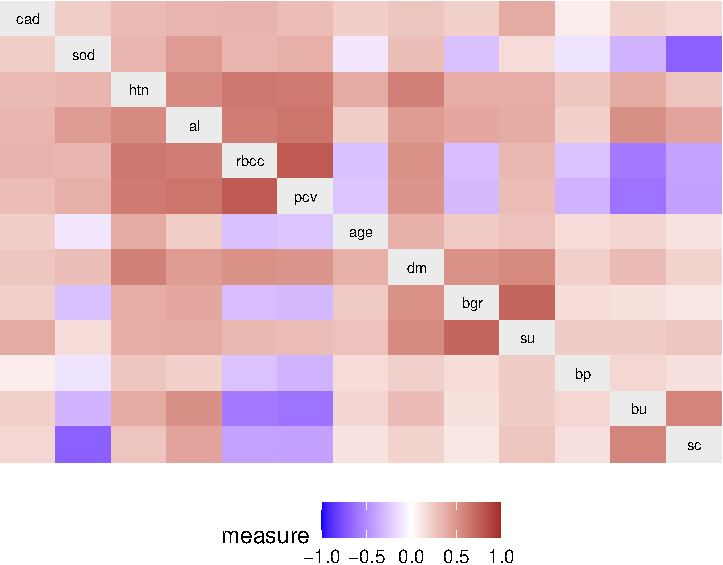
\includegraphics{rj_paper_files/figure-latex/assoc-heatmap-1} 

}

\caption[Association matrix display for penguins data showing Pearson's correlation for numeric variable pairs, canonical correlation for mixed variable pairs and categorical variable pairs]{Association matrix display for penguins data showing Pearson's correlation for numeric variable pairs, canonical correlation for mixed variable pairs and categorical variable pairs.}\label{fig:assoc-heatmap}
\end{figure}
\end{Schunk}

We can also calculate multiple association measures for all the variable
pairs in the dataset and compare them. This will help in finding out
pairs of variables with a high difference among different measures and
one can investigate these bivariate relationships in more detail. The
\texttt{pairwise\_summary\_plot} function can be used to compare various
measures using the matrix layout. It plots multiple measures among the
variable pairs as bars, where each bar represents one measure of
association. Figure \ref{fig:compare-matrix} shows a matrix layout
comparing Pearson's and Spearman's correlation coefficient for the
numeric variable pairs in \texttt{penguins} data.

\begin{Schunk}
\begin{figure}

{\centering 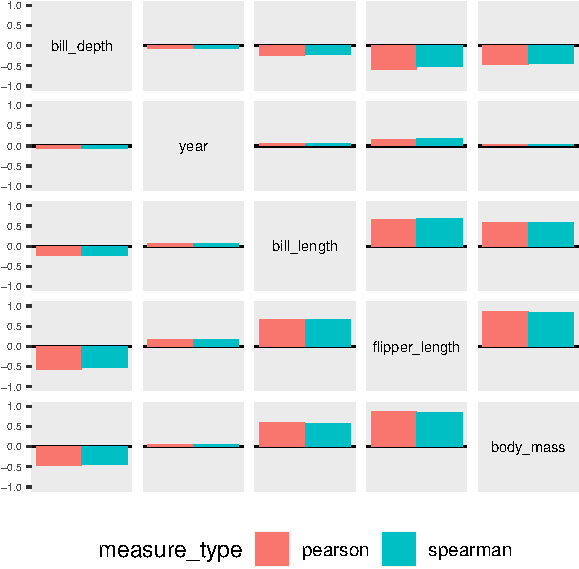
\includegraphics{rj_paper_files/figure-latex/compare-matrix-1} 

}

\caption[Matrix display comparing Pearson's and Spearman's correlation coefficient]{Matrix display comparing Pearson's and Spearman's correlation coefficient. All the variable pairs have similar values for both correlations.}\label{fig:compare-matrix}
\end{figure}
\end{Schunk}

In addition to matrix layout, we can also use linear layouts for
comparing multiple measures. Figure \ref{fig:compare-linear} shows a
linear layout comparing multiple association measures for all the
variable pairs in the penguins data. Linear layouts seems to be more
suitable when comparing high number of association measures.

\begin{Schunk}
\begin{figure}

{\centering 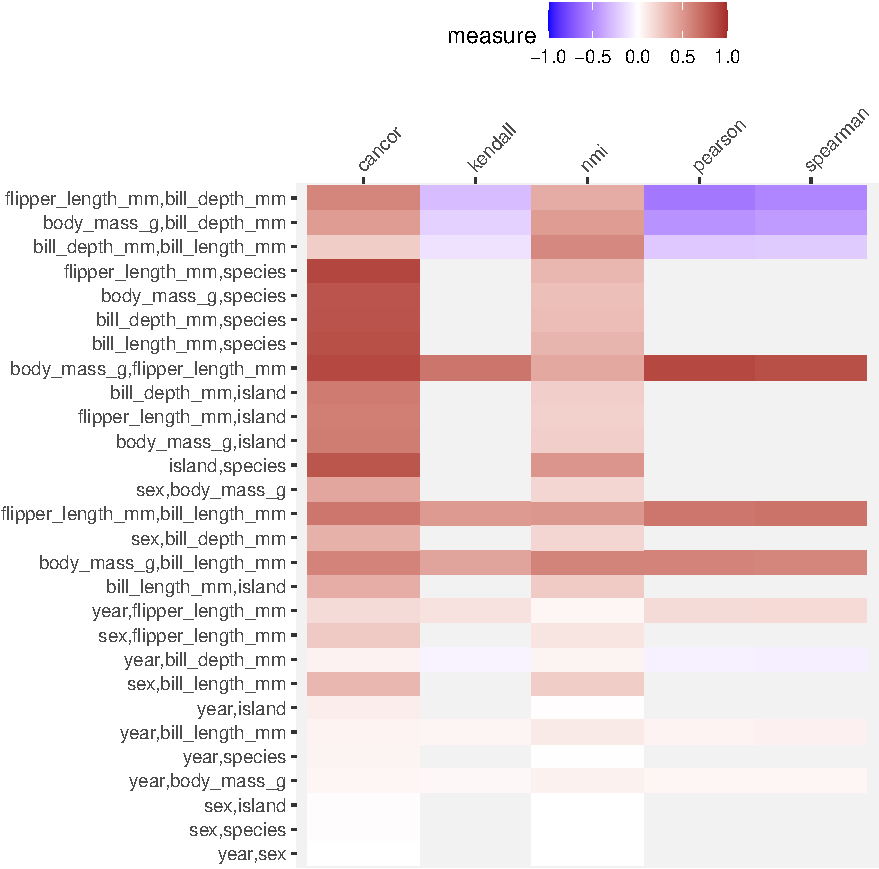
\includegraphics{rj_paper_files/figure-latex/compare-linear-1} 

}

\caption[Comparing multiple association measures using a linear layout]{Comparing multiple association measures using a linear layout. The display has variable pairs on the Y-axis and association measures on the X-axis. The cell corresponding to a variable pair and an association measure has been colored grey showing that the measure is not defined for corresponding pair.}\label{fig:compare-linear}
\end{figure}
\end{Schunk}

\hypertarget{visualising-conditional-association}{%
\subsection{Visualising Conditional
Association}\label{visualising-conditional-association}}

The package includes a function \texttt{calc\_assoc\_by} which
calculates the pairwise association at different levels of a categorical
conditioning variable. This helps in finding out interesting variable
triples which can be explored further prior to modeling. Figure
\ref{fig:cond-assoc} shows a conditional association plot for the
\texttt{penguins} data. Each cell corresponding to a variable pair shows
three bars which correspond to the association measure (Pearson's
correlation for numeric pair and Normalized mutual information for other
combination of variables) calculated at the levels of conditioning
variable \texttt{island}. The dashed line represents the overall
association measure. The plot shows that there is a high value for
normalised mutual information between bill\_length\_mm and species for
the penguins which lived in \texttt{Biscoe} island compared to the
penguins which lived in \texttt{Dream} island. It can also be seen that
the cell corresponding to variable pair flipper\_length\_mm and
bill\_depth\_mm has a high negative overall Pearson's correlation and
for the penguins which lived in \texttt{Biscoe} island but positive
correlation for penguins which lived in \texttt{Dream} and
\texttt{Torgersen} island. This is an instance of Simpson's paradox
which can be taken into account during the modeling step.

\begin{Schunk}
\begin{figure}

{\centering 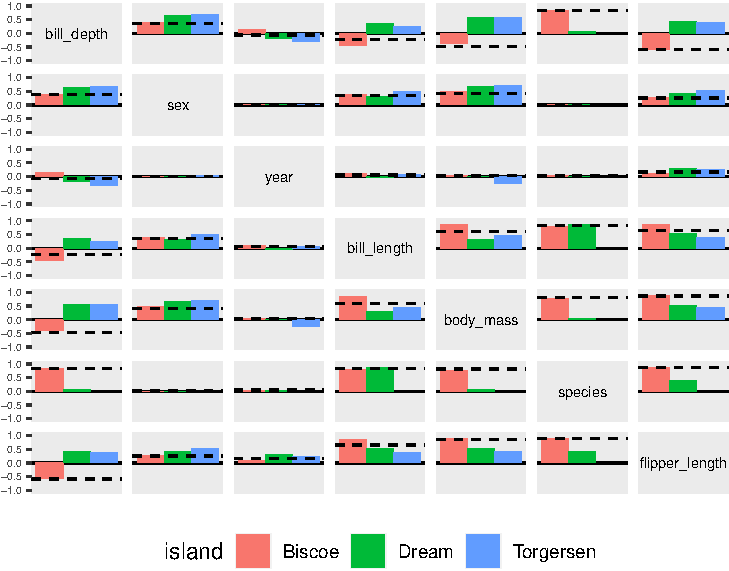
\includegraphics{rj_paper_files/figure-latex/cond-assoc-1} 

}

\caption[Conditional Association plot for penguins data showing Pearson's correlation for numeric pairs and normalised mutual information for categorical or mixed pairs]{Conditional Association plot for penguins data showing Pearson's correlation for numeric pairs and normalised mutual information for categorical or mixed pairs. The bars in each cell represent the value for asssociation measure colored by the conditioning variable `island`. The dashed line in each cell represents overall value of the association measure.}\label{fig:cond-assoc}
\end{figure}
\end{Schunk}

We also provide a functionality for highlighting interesting patterns
like Simpson's paradox. Figure \ref{fig:cond-assoc-sp} shows the matrix
plot with highlighted cells for the variable pairs where Simpson's
paradox is present.

\begin{Schunk}
\begin{figure}

{\centering 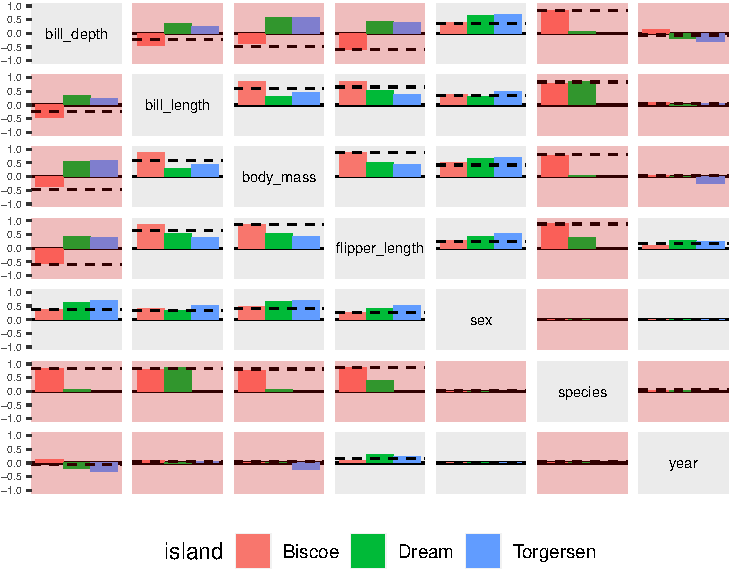
\includegraphics{rj_paper_files/figure-latex/cond-assoc-sp-1} 

}

\caption[Conditional Association plot with examples of Simpson's paradox]{Conditional Association plot with examples of Simpson's paradox}\label{fig:cond-assoc-sp}
\end{figure}
\end{Schunk}

The cells can also be highlighted on the basis of a score calculated by
the user. This can be done by providing a dataframe with pairs of
variables to highlight and a score for highlighting variable pairs. The
cells with high score will have a thicker border compared to cells with
low score. Figure \ref{fig:cond-assoc-manual} shows highlighted cells on
the basis of a score provided for a subset of variable pairs.

\begin{Schunk}
\begin{figure}

{\centering 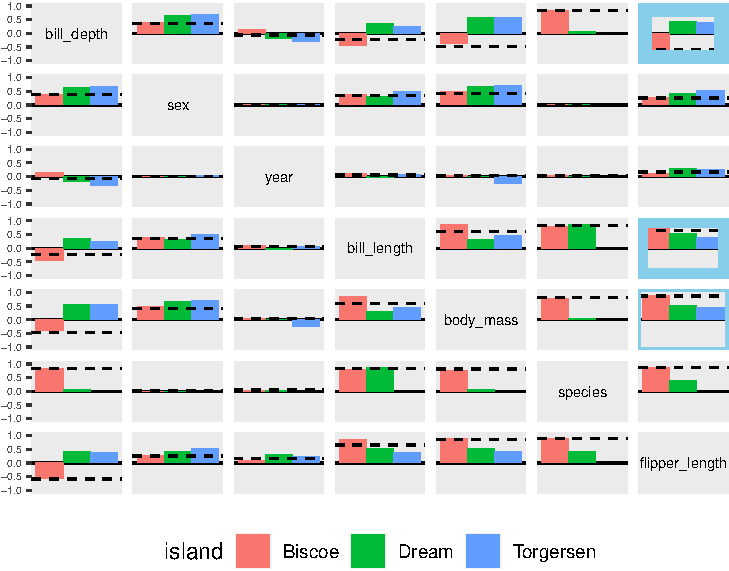
\includegraphics{rj_paper_files/figure-latex/cond-assoc-manual-1} 

}

\caption[Conditional Association plot with manual highlighting]{Conditional Association plot with manual highlighting}\label{fig:cond-assoc-manual}
\end{figure}
\end{Schunk}

We can also use linear layouts for displaying conditional association.
Figure \ref{fig:linear-cond-assoc} shows a funnel-like linear display
for conditional association measures with all the variable pairs on the
y-axis, the value of association measure on x-axis and color of the
points representing the level of the grouping variable. The linear
layout becomes more useful over the matrix layout when the number of
variables and number of levels of grouping variable are high.

\begin{Schunk}
\begin{figure}

{\centering 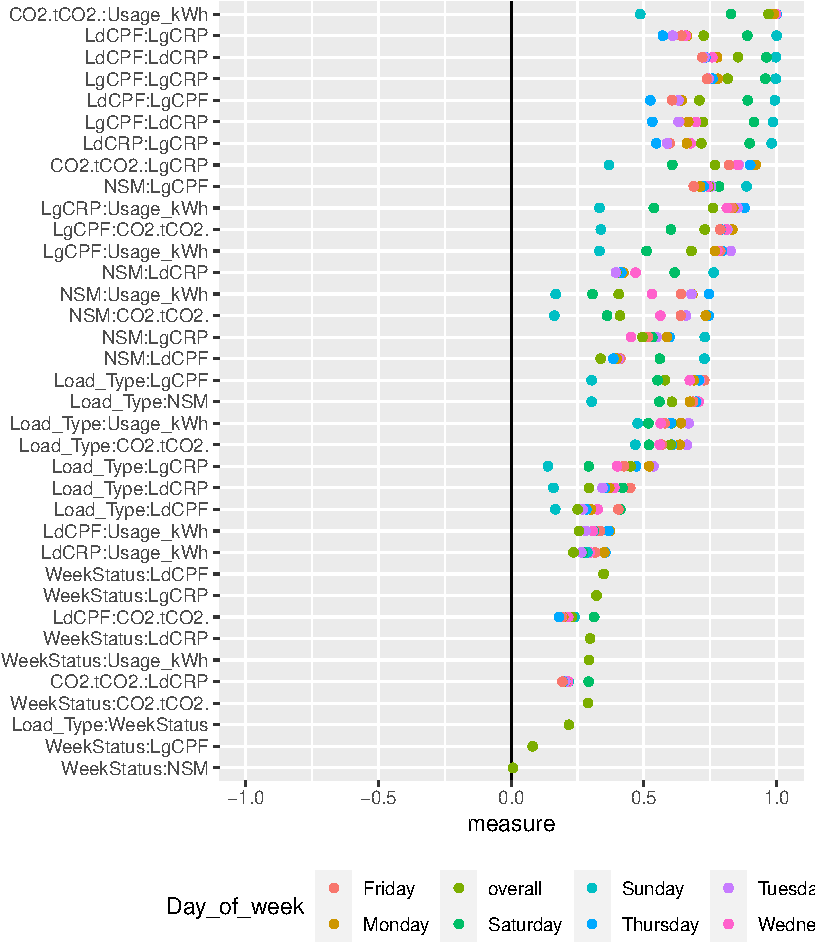
\includegraphics{rj_paper_files/figure-latex/linear-cond-assoc-1} 

}

\caption[Conditional Association plot using linear layout.The display has variable pairs on the Y-axis and the value of association measures on the X-axis]{Conditional Association plot using linear layout.The display has variable pairs on the Y-axis and the value of association measures on the X-axis. The points corresponding to every variable pair represents the value of association measure for different levels of the conditioning variable and the overall value of association measure.}\label{fig:linear-cond-assoc}
\end{figure}
\end{Schunk}

\bibliography{RJreferences.bib}

\address{%
Amit Chinwan\\
Maynooth University\\%
Hamilton Institute\\ Maynooth, Ireland\\
%
%
%
\href{mailto:amit.chinwan.2019@mumail.ie}{\nolinkurl{amit.chinwan.2019@mumail.ie}}%
}

\address{%
Catherine Hurley\\
Maynooth University\\%
Department of Mathematics and Statistics\\ Maynooth, Ireland\\
%
%
%
\href{mailto:catherine.hurley@mu.ie}{\nolinkurl{catherine.hurley@mu.ie}}%
}
